\documentclass[1p]{elsarticle_modified}
%\bibliographystyle{elsarticle-num}

%\usepackage[colorlinks]{hyperref}
%\usepackage{abbrmath_seonhwa} %\Abb, \Ascr, \Acal ,\Abf, \Afrak
\usepackage{amsfonts}
\usepackage{amssymb}
\usepackage{amsmath}
\usepackage{amsthm}
\usepackage{scalefnt}
\usepackage{amsbsy}
\usepackage{kotex}
\usepackage{caption}
\usepackage{subfig}
\usepackage{color}
\usepackage{graphicx}
\usepackage{xcolor} %% white, black, red, green, blue, cyan, magenta, yellow
\usepackage{float}
\usepackage{setspace}
\usepackage{hyperref}

\usepackage{tikz}
\usetikzlibrary{arrows}

\usepackage{multirow}
\usepackage{array} % fixed length table
\usepackage{hhline}

%%%%%%%%%%%%%%%%%%%%%
\makeatletter
\renewcommand*\env@matrix[1][\arraystretch]{%
	\edef\arraystretch{#1}%
	\hskip -\arraycolsep
	\let\@ifnextchar\new@ifnextchar
	\array{*\c@MaxMatrixCols c}}
\makeatother %https://tex.stackexchange.com/questions/14071/how-can-i-increase-the-line-spacing-in-a-matrix
%%%%%%%%%%%%%%%

\usepackage[normalem]{ulem}

\newcommand{\msout}[1]{\ifmmode\text{\sout{\ensuremath{#1}}}\else\sout{#1}\fi}
%SOURCE: \msout is \stkout macro in https://tex.stackexchange.com/questions/20609/strikeout-in-math-mode

\newcommand{\cancel}[1]{
	\ifmmode
	{\color{red}\msout{#1}}
	\else
	{\color{red}\sout{#1}}
	\fi
}

\newcommand{\add}[1]{
	{\color{blue}\uwave{#1}}
}

\newcommand{\replace}[2]{
	\ifmmode
	{\color{red}\msout{#1}}{\color{blue}\uwave{#2}}
	\else
	{\color{red}\sout{#1}}{\color{blue}\uwave{#2}}
	\fi
}

\newcommand{\Sol}{\mathcal{S}} %segment
\newcommand{\D}{D} %diagram
\newcommand{\A}{\mathcal{A}} %arc


%%%%%%%%%%%%%%%%%%%%%%%%%%%%%5 test

\def\sl{\operatorname{\textup{SL}}(2,\Cbb)}
\def\psl{\operatorname{\textup{PSL}}(2,\Cbb)}
\def\quan{\mkern 1mu \triangleright \mkern 1mu}

\theoremstyle{definition}
\newtheorem{thm}{Theorem}[section]
\newtheorem{prop}[thm]{Proposition}
\newtheorem{lem}[thm]{Lemma}
\newtheorem{ques}[thm]{Question}
\newtheorem{cor}[thm]{Corollary}
\newtheorem{defn}[thm]{Definition}
\newtheorem{exam}[thm]{Example}
\newtheorem{rmk}[thm]{Remark}
\newtheorem{alg}[thm]{Algorithm}

\newcommand{\I}{\sqrt{-1}}
\begin{document}

%\begin{frontmatter}
%
%\title{Boundary parabolic representations of knots up to 8 crossings}
%
%%% Group authors per affiliation:
%\author{Yunhi Cho} 
%\address{Department of Mathematics, University of Seoul, Seoul, Korea}
%\ead{yhcho@uos.ac.kr}
%
%
%\author{Seonhwa Kim} %\fnref{s_kim}}
%\address{Center for Geometry and Physics, Institute for Basic Science, Pohang, 37673, Korea}
%\ead{ryeona17@ibs.re.kr}
%
%\author{Hyuk Kim}
%\address{Department of Mathematical Sciences, Seoul National University, Seoul 08826, Korea}
%\ead{hyukkim@snu.ac.kr}
%
%\author{Seokbeom Yoon}
%\address{Department of Mathematical Sciences, Seoul National University, Seoul, 08826,  Korea}
%\ead{sbyoon15@snu.ac.kr}
%
%\begin{abstract}
%We find all boundary parabolic representation of knots up to 8 crossings.
%
%\end{abstract}
%\begin{keyword}
%    \MSC[2010] 57M25 
%\end{keyword}
%
%\end{frontmatter}

%\linenumbers
%\tableofcontents
%
\newcommand\colored[1]{\textcolor{white}{\rule[-0.35ex]{0.8em}{1.4ex}}\kern-0.8em\color{red} #1}%
%\newcommand\colored[1]{\textcolor{white}{ #1}\kern-2.17ex	\textcolor{white}{ #1}\kern-1.81ex	\textcolor{white}{ #1}\kern-2.15ex\color{red}#1	}

{\Large $\underline{12a_{0322}~(K12a_{0322})}$}

\setlength{\tabcolsep}{10pt}
\renewcommand{\arraystretch}{1.6}
\vspace{1cm}\begin{tabular}{m{100pt}>{\centering\arraybackslash}m{274pt}}
\multirow{5}{120pt}{
	\centering
	\includegraphics[width=112pt]{../../../GIT/diagram.site/Diagrams/png/1123_12a_0322.png}\\
\ \ \ A knot diagram\footnotemark}&
\allowdisplaybreaks
\textbf{Linearized knot diagam} \\
\cline{2-2}
 &
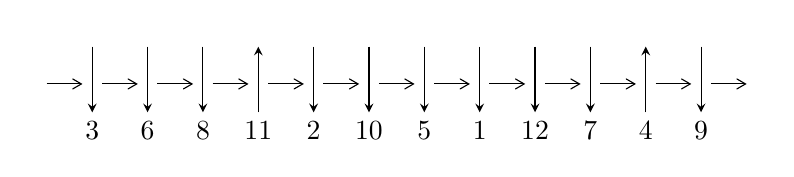
\begin{tikzpicture}[x=20pt, y=17pt]
	% nodes
	\node (C0) at (0, 0) {};
	\node (C1) at (1, 0) {};
	\node (C1U) at (1, +1) {};
	\node (C1D) at (1, -1) {3};

	\node (C2) at (2, 0) {};
	\node (C2U) at (2, +1) {};
	\node (C2D) at (2, -1) {6};

	\node (C3) at (3, 0) {};
	\node (C3U) at (3, +1) {};
	\node (C3D) at (3, -1) {8};

	\node (C4) at (4, 0) {};
	\node (C4U) at (4, +1) {};
	\node (C4D) at (4, -1) {11};

	\node (C5) at (5, 0) {};
	\node (C5U) at (5, +1) {};
	\node (C5D) at (5, -1) {2};

	\node (C6) at (6, 0) {};
	\node (C6U) at (6, +1) {};
	\node (C6D) at (6, -1) {10};

	\node (C7) at (7, 0) {};
	\node (C7U) at (7, +1) {};
	\node (C7D) at (7, -1) {5};

	\node (C8) at (8, 0) {};
	\node (C8U) at (8, +1) {};
	\node (C8D) at (8, -1) {1};

	\node (C9) at (9, 0) {};
	\node (C9U) at (9, +1) {};
	\node (C9D) at (9, -1) {12};

	\node (C10) at (10, 0) {};
	\node (C10U) at (10, +1) {};
	\node (C10D) at (10, -1) {7};

	\node (C11) at (11, 0) {};
	\node (C11U) at (11, +1) {};
	\node (C11D) at (11, -1) {4};

	\node (C12) at (12, 0) {};
	\node (C12U) at (12, +1) {};
	\node (C12D) at (12, -1) {9};
	\node (C13) at (13, 0) {};

	% arrows
	\draw[->,>={angle 60}]
	(C0) edge (C1) (C1) edge (C2) (C2) edge (C3) (C3) edge (C4) (C4) edge (C5) (C5) edge (C6) (C6) edge (C7) (C7) edge (C8) (C8) edge (C9) (C9) edge (C10) (C10) edge (C11) (C11) edge (C12) (C12) edge (C13) ;	\draw[->,>=stealth]
	(C1U) edge (C1D) (C2U) edge (C2D) (C3U) edge (C3D) (C4D) edge (C4U) (C5U) edge (C5D) (C6U) edge (C6D) (C7U) edge (C7D) (C8U) edge (C8D) (C9U) edge (C9D) (C10U) edge (C10D) (C11D) edge (C11U) (C12U) edge (C12D) ;
	\end{tikzpicture} \\
\hhline{~~} \\& 
\textbf{Solving Sequence} \\ \cline{2-2} 
 &
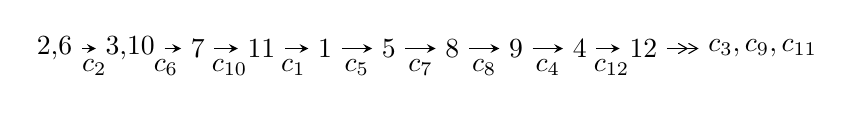
\begin{tikzpicture}[x=23pt, y=7pt]
	% node
	\node (A0) at (-1/8, 0) {2,6};
	\node (A1) at (17/16, 0) {3,10};
	\node (A2) at (17/8, 0) {7};
	\node (A3) at (25/8, 0) {11};
	\node (A4) at (33/8, 0) {1};
	\node (A5) at (41/8, 0) {5};
	\node (A6) at (49/8, 0) {8};
	\node (A7) at (57/8, 0) {9};
	\node (A8) at (65/8, 0) {4};
	\node (A9) at (73/8, 0) {12};
	\node (C1) at (1/2, -1) {$c_{2}$};
	\node (C2) at (13/8, -1) {$c_{6}$};
	\node (C3) at (21/8, -1) {$c_{10}$};
	\node (C4) at (29/8, -1) {$c_{1}$};
	\node (C5) at (37/8, -1) {$c_{5}$};
	\node (C6) at (45/8, -1) {$c_{7}$};
	\node (C7) at (53/8, -1) {$c_{8}$};
	\node (C8) at (61/8, -1) {$c_{4}$};
	\node (C9) at (69/8, -1) {$c_{12}$};
	\node (A10) at (11, 0) {$c_{3},c_{9},c_{11}$};

	% edge
	\draw[->,>=stealth]	
	(A0) edge (A1) (A1) edge (A2) (A2) edge (A3) (A3) edge (A4) (A4) edge (A5) (A5) edge (A6) (A6) edge (A7) (A7) edge (A8) (A8) edge (A9) ;
	\draw[->>,>={angle 60}]	
	(A9) edge (A10);
\end{tikzpicture} \\ 

\end{tabular} \\

\footnotetext{
The image of knot diagram is generated by the software ``\textbf{Draw programme}" developed by Andrew Bartholomew(\url{http://www.layer8.co.uk/maths/draw/index.htm\#Running-draw}), where we modified some parts for our purpose(\url{https://github.com/CATsTAILs/LinksPainter}).
}\phantom \\ \newline 
\centering \textbf{Ideals for irreducible components\footnotemark of $X_{\text{par}}$} 
 
\begin{align*}
I^u_{1}&=\langle 
-8.21898\times10^{219} u^{119}+4.76957\times10^{220} u^{118}+\cdots+4.63553\times10^{219} b+9.71727\times10^{220},\\
\phantom{I^u_{1}}&\phantom{= \langle  }-6.19206\times10^{220} u^{119}+3.81909\times10^{221} u^{118}+\cdots+3.24487\times10^{220} a+1.01535\times10^{222},\\
\phantom{I^u_{1}}&\phantom{= \langle  }u^{120}-7 u^{119}+\cdots-322 u+28\rangle \\
I^u_{2}&=\langle 
11 u^{27}-7 u^{26}+\cdots+b+9,\;21 u^{27}-14 u^{26}+\cdots+a+26,\;u^{28}-7 u^{26}+\cdots-7 u^2+1\rangle \\
\\
\end{align*}
\raggedright * 2 irreducible components of $\dim_{\mathbb{C}}=0$, with total 148 representations.\\
\footnotetext{All coefficients of polynomials are rational numbers. But the coefficients are sometimes approximated in decimal forms when there is not enough margin.}
\newpage
\renewcommand{\arraystretch}{1}
\centering \section*{I. $I^u_{1}= \langle -8.22\times10^{219} u^{119}+4.77\times10^{220} u^{118}+\cdots+4.64\times10^{219} b+9.72\times10^{220},\;-6.19\times10^{220} u^{119}+3.82\times10^{221} u^{118}+\cdots+3.24\times10^{220} a+1.02\times10^{222},\;u^{120}-7 u^{119}+\cdots-322 u+28 \rangle$}
\flushleft \textbf{(i) Arc colorings}\\
\begin{tabular}{m{7pt} m{180pt} m{7pt} m{180pt} }
\flushright $a_{2}=$&$\begin{pmatrix}1\\0\end{pmatrix}$ \\
\flushright $a_{6}=$&$\begin{pmatrix}0\\u\end{pmatrix}$ \\
\flushright $a_{3}=$&$\begin{pmatrix}1\\u^2\end{pmatrix}$ \\
\flushright $a_{10}=$&$\begin{pmatrix}1.90826 u^{119}-11.7696 u^{118}+\cdots+411.586 u-31.2907\\1.77304 u^{119}-10.2892 u^{118}+\cdots+249.202 u-20.9626\end{pmatrix}$ \\
\flushright $a_{7}=$&$\begin{pmatrix}1.44392 u^{119}-9.00588 u^{118}+\cdots+407.842 u-43.3368\\1.81874 u^{119}-11.5795 u^{118}+\cdots+548.122 u-51.0257\end{pmatrix}$ \\
\flushright $a_{11}=$&$\begin{pmatrix}0.378475 u^{119}-1.79691 u^{118}+\cdots-126.882 u+17.7038\\0.145425 u^{119}-0.0262595 u^{118}+\cdots-227.960 u+23.7574\end{pmatrix}$ \\
\flushright $a_{1}=$&$\begin{pmatrix}- u^2+1\\- u^4\end{pmatrix}$ \\
\flushright $a_{5}=$&$\begin{pmatrix}u\\u\end{pmatrix}$ \\
\flushright $a_{8}=$&$\begin{pmatrix}1.88512 u^{119}-11.3227 u^{118}+\cdots+402.195 u-41.9332\\2.25994 u^{119}-13.8963 u^{118}+\cdots+542.476 u-49.6221\end{pmatrix}$ \\
\flushright $a_{9}=$&$\begin{pmatrix}1.46394 u^{119}-9.13960 u^{118}+\cdots+425.876 u-45.4088\\1.86261 u^{119}-11.8211 u^{118}+\cdots+537.652 u-50.5064\end{pmatrix}$ \\
\flushright $a_{4}=$&$\begin{pmatrix}-0.741655 u^{119}+4.42736 u^{118}+\cdots-216.390 u+18.8365\\-0.0128759 u^{119}-0.437223 u^{118}+\cdots+131.410 u-13.0382\end{pmatrix}$ \\
\flushright $a_{12}=$&$\begin{pmatrix}0.550241 u^{119}-3.00283 u^{118}+\cdots+75.1762 u-3.88524\\-0.0827609 u^{119}+1.69612 u^{118}+\cdots-314.707 u+31.3255\end{pmatrix}$\\&\end{tabular}
\flushleft \textbf{(ii) Obstruction class $= -1$}\\~\\
\flushleft \textbf{(iii) Cusp Shapes $= -1.89337 u^{119}+12.9136 u^{118}+\cdots-1169.14 u+100.982$}\\~\\
\newpage\renewcommand{\arraystretch}{1}
\flushleft \textbf{(iv) u-Polynomials at the component}\newline \\
\begin{tabular}{m{50pt}|m{274pt}}
Crossings & \hspace{64pt}u-Polynomials at each crossing \\
\hline $$\begin{aligned}c_{1}\end{aligned}$$&$\begin{aligned}
&u^{120}+49 u^{119}+\cdots+44492 u+784
\end{aligned}$\\
\hline $$\begin{aligned}c_{2},c_{5}\end{aligned}$$&$\begin{aligned}
&u^{120}+7 u^{119}+\cdots+322 u+28
\end{aligned}$\\
\hline $$\begin{aligned}c_{3}\end{aligned}$$&$\begin{aligned}
&u^{120}+u^{119}+\cdots+3289256 u-546677
\end{aligned}$\\
\hline $$\begin{aligned}c_{4},c_{11}\end{aligned}$$&$\begin{aligned}
&u^{120}-3 u^{119}+\cdots-47904 u+17881
\end{aligned}$\\
\hline $$\begin{aligned}c_{6},c_{10}\end{aligned}$$&$\begin{aligned}
&u^{120}-3 u^{119}+\cdots-110801 u-32041
\end{aligned}$\\
\hline $$\begin{aligned}c_{7}\end{aligned}$$&$\begin{aligned}
&u^{120}-3 u^{119}+\cdots+8809070 u-639127
\end{aligned}$\\
\hline $$\begin{aligned}c_{8},c_{9},c_{12}\end{aligned}$$&$\begin{aligned}
&u^{120}-4 u^{119}+\cdots-116 u+7
\end{aligned}$\\
\hline
\end{tabular}\\~\\
\newpage\renewcommand{\arraystretch}{1}
\flushleft \textbf{(v) Riley Polynomials at the component}\newline \\
\begin{tabular}{m{50pt}|m{274pt}}
Crossings & \hspace{64pt}Riley Polynomials at each crossing \\
\hline $$\begin{aligned}c_{1}\end{aligned}$$&$\begin{aligned}
&y^{120}+59 y^{119}+\cdots-985957616 y+614656
\end{aligned}$\\
\hline $$\begin{aligned}c_{2},c_{5}\end{aligned}$$&$\begin{aligned}
&y^{120}-49 y^{119}+\cdots-44492 y+784
\end{aligned}$\\
\hline $$\begin{aligned}c_{3}\end{aligned}$$&$\begin{aligned}
&y^{120}+21 y^{119}+\cdots+9174574703856 y+298855742329
\end{aligned}$\\
\hline $$\begin{aligned}c_{4},c_{11}\end{aligned}$$&$\begin{aligned}
&y^{120}+89 y^{119}+\cdots-4994108976 y+319730161
\end{aligned}$\\
\hline $$\begin{aligned}c_{6},c_{10}\end{aligned}$$&$\begin{aligned}
&y^{120}-81 y^{119}+\cdots+2923581045 y+1026625681
\end{aligned}$\\
\hline $$\begin{aligned}c_{7}\end{aligned}$$&$\begin{aligned}
&y^{120}-33 y^{119}+\cdots-17599469821274 y+408483322129
\end{aligned}$\\
\hline $$\begin{aligned}c_{8},c_{9},c_{12}\end{aligned}$$&$\begin{aligned}
&y^{120}+118 y^{119}+\cdots+1566 y+49
\end{aligned}$\\
\hline
\end{tabular}\\~\\
\newpage\flushleft \textbf{(vi) Complex Volumes and Cusp Shapes}
$$\begin{array}{c|c|c}  
\text{Solutions to }I^u_{1}& \I (\text{vol} + \sqrt{-1}CS) & \text{Cusp shape}\\
 \hline 
\begin{aligned}
u &= \phantom{-}0.794130 + 0.592091 I \\
a &= -1.036180 + 0.139905 I \\
b &= -2.73059 + 1.18931 I\end{aligned}
 & \phantom{-}5.76528 - 4.26197 I & \phantom{-0.000000 } 0 \\ \hline\begin{aligned}
u &= \phantom{-}0.794130 - 0.592091 I \\
a &= -1.036180 - 0.139905 I \\
b &= -2.73059 - 1.18931 I\end{aligned}
 & \phantom{-}5.76528 + 4.26197 I & \phantom{-0.000000 } 0 \\ \hline\begin{aligned}
u &= -0.811711 + 0.559362 I \\
a &= \phantom{-}0.43814 + 1.54982 I \\
b &= -0.135332 + 0.657514 I\end{aligned}
 & -1.05368 - 2.08033 I & \phantom{-0.000000 } 0 \\ \hline\begin{aligned}
u &= -0.811711 - 0.559362 I \\
a &= \phantom{-}0.43814 - 1.54982 I \\
b &= -0.135332 - 0.657514 I\end{aligned}
 & -1.05368 + 2.08033 I & \phantom{-0.000000 } 0 \\ \hline\begin{aligned}
u &= \phantom{-}0.795910 + 0.567712 I \\
a &= \phantom{-}0.636281 + 0.221317 I \\
b &= \phantom{-}0.451032 - 0.933379 I\end{aligned}
 & -0.64341 - 1.79431 I & \phantom{-0.000000 } 0 \\ \hline\begin{aligned}
u &= \phantom{-}0.795910 - 0.567712 I \\
a &= \phantom{-}0.636281 - 0.221317 I \\
b &= \phantom{-}0.451032 + 0.933379 I\end{aligned}
 & -0.64341 + 1.79431 I & \phantom{-0.000000 } 0 \\ \hline\begin{aligned}
u &= \phantom{-}0.500076 + 0.838852 I \\
a &= -0.21069 + 1.40177 I \\
b &= \phantom{-}0.066259 - 0.537185 I\end{aligned}
 & -3.58790 + 7.84949 I & \phantom{-0.000000 } 0 \\ \hline\begin{aligned}
u &= \phantom{-}0.500076 - 0.838852 I \\
a &= -0.21069 - 1.40177 I \\
b &= \phantom{-}0.066259 + 0.537185 I\end{aligned}
 & -3.58790 - 7.84949 I & \phantom{-0.000000 } 0 \\ \hline\begin{aligned}
u &= -0.704119 + 0.669771 I \\
a &= \phantom{-}0.687117 - 0.261579 I \\
b &= \phantom{-}0.614214 - 0.164025 I\end{aligned}
 & \phantom{-}2.81216 + 1.01478 I & \phantom{-0.000000 } 0 \\ \hline\begin{aligned}
u &= -0.704119 - 0.669771 I \\
a &= \phantom{-}0.687117 + 0.261579 I \\
b &= \phantom{-}0.614214 + 0.164025 I\end{aligned}
 & \phantom{-}2.81216 - 1.01478 I & \phantom{-0.000000 } 0\\
 \hline 
 \end{array}$$\newpage$$\begin{array}{c|c|c}  
\text{Solutions to }I^u_{1}& \I (\text{vol} + \sqrt{-1}CS) & \text{Cusp shape}\\
 \hline 
\begin{aligned}
u &= -1.022580 + 0.152770 I \\
a &= -1.090080 - 0.430824 I \\
b &= -3.13345 - 0.41355 I\end{aligned}
 & -7.07823 - 1.36704 I & \phantom{-0.000000 } 0 \\ \hline\begin{aligned}
u &= -1.022580 - 0.152770 I \\
a &= -1.090080 + 0.430824 I \\
b &= -3.13345 + 0.41355 I\end{aligned}
 & -7.07823 + 1.36704 I & \phantom{-0.000000 } 0 \\ \hline\begin{aligned}
u &= \phantom{-}0.876865 + 0.373837 I \\
a &= -1.10967 + 1.33609 I \\
b &= -1.79299 + 1.08629 I\end{aligned}
 & -2.47601 + 2.18680 I & \phantom{-0.000000 } 0 \\ \hline\begin{aligned}
u &= \phantom{-}0.876865 - 0.373837 I \\
a &= -1.10967 - 1.33609 I \\
b &= -1.79299 - 1.08629 I\end{aligned}
 & -2.47601 - 2.18680 I & \phantom{-0.000000 } 0 \\ \hline\begin{aligned}
u &= \phantom{-}0.522358 + 0.796481 I \\
a &= \phantom{-}1.166810 + 0.561303 I \\
b &= \phantom{-}1.068930 + 0.135249 I\end{aligned}
 & \phantom{-}6.72132 + 5.58019 I & \phantom{-0.000000 } 0 \\ \hline\begin{aligned}
u &= \phantom{-}0.522358 - 0.796481 I \\
a &= \phantom{-}1.166810 - 0.561303 I \\
b &= \phantom{-}1.068930 - 0.135249 I\end{aligned}
 & \phantom{-}6.72132 - 5.58019 I & \phantom{-0.000000 } 0 \\ \hline\begin{aligned}
u &= -0.941729 + 0.027426 I \\
a &= -0.341445 - 0.791610 I \\
b &= \phantom{-}0.100180 - 1.011340 I\end{aligned}
 & -4.48747 - 1.81759 I & \phantom{-0.000000 } 0 \\ \hline\begin{aligned}
u &= -0.941729 - 0.027426 I \\
a &= -0.341445 + 0.791610 I \\
b &= \phantom{-}0.100180 + 1.011340 I\end{aligned}
 & -4.48747 + 1.81759 I & \phantom{-0.000000 } 0 \\ \hline\begin{aligned}
u &= -0.901163 + 0.562425 I \\
a &= \phantom{-}1.59113 - 0.13593 I \\
b &= \phantom{-}2.59861 + 0.39022 I\end{aligned}
 & -1.34992 + 6.56399 I & \phantom{-0.000000 } 0 \\ \hline\begin{aligned}
u &= -0.901163 - 0.562425 I \\
a &= \phantom{-}1.59113 + 0.13593 I \\
b &= \phantom{-}2.59861 - 0.39022 I\end{aligned}
 & -1.34992 - 6.56399 I & \phantom{-0.000000 } 0\\
 \hline 
 \end{array}$$\newpage$$\begin{array}{c|c|c}  
\text{Solutions to }I^u_{1}& \I (\text{vol} + \sqrt{-1}CS) & \text{Cusp shape}\\
 \hline 
\begin{aligned}
u &= -0.755449 + 0.535537 I \\
a &= \phantom{-}0.802382 + 0.494497 I \\
b &= \phantom{-}3.33001 + 0.42016 I\end{aligned}
 & \phantom{-}5.39303 - 1.61910 I & \phantom{-0.000000 } 0 \\ \hline\begin{aligned}
u &= -0.755449 - 0.535537 I \\
a &= \phantom{-}0.802382 - 0.494497 I \\
b &= \phantom{-}3.33001 - 0.42016 I\end{aligned}
 & \phantom{-}5.39303 + 1.61910 I & \phantom{-0.000000 } 0 \\ \hline\begin{aligned}
u &= -0.773230 + 0.493848 I \\
a &= -0.691757 - 0.832970 I \\
b &= -0.91976 + 1.11074 I\end{aligned}
 & -1.07276 + 1.31581 I & \phantom{-0.000000 } 0 \\ \hline\begin{aligned}
u &= -0.773230 - 0.493848 I \\
a &= -0.691757 + 0.832970 I \\
b &= -0.91976 - 1.11074 I\end{aligned}
 & -1.07276 - 1.31581 I & \phantom{-0.000000 } 0 \\ \hline\begin{aligned}
u &= \phantom{-}1.008900 + 0.403302 I \\
a &= \phantom{-}1.24638 - 0.80340 I \\
b &= \phantom{-}2.06463 - 0.73656 I\end{aligned}
 & -6.67226 - 1.10006 I & \phantom{-0.000000 } 0 \\ \hline\begin{aligned}
u &= \phantom{-}1.008900 - 0.403302 I \\
a &= \phantom{-}1.24638 + 0.80340 I \\
b &= \phantom{-}2.06463 + 0.73656 I\end{aligned}
 & -6.67226 + 1.10006 I & \phantom{-0.000000 } 0 \\ \hline\begin{aligned}
u &= -0.614899 + 0.899173 I \\
a &= -0.812781 + 0.037535 I \\
b &= -0.927483 + 0.068797 I\end{aligned}
 & \phantom{-}9.37495 - 0.63348 I & \phantom{-0.000000 } 0 \\ \hline\begin{aligned}
u &= -0.614899 - 0.899173 I \\
a &= -0.812781 - 0.037535 I \\
b &= -0.927483 - 0.068797 I\end{aligned}
 & \phantom{-}9.37495 + 0.63348 I & \phantom{-0.000000 } 0 \\ \hline\begin{aligned}
u &= \phantom{-}0.801649 + 0.737933 I \\
a &= -0.132730 + 1.004280 I \\
b &= \phantom{-}0.791265 + 0.400595 I\end{aligned}
 & \phantom{-}5.97079 + 0.59954 I & \phantom{-0.000000 } 0 \\ \hline\begin{aligned}
u &= \phantom{-}0.801649 - 0.737933 I \\
a &= -0.132730 - 1.004280 I \\
b &= \phantom{-}0.791265 - 0.400595 I\end{aligned}
 & \phantom{-}5.97079 - 0.59954 I & \phantom{-0.000000 } 0\\
 \hline 
 \end{array}$$\newpage$$\begin{array}{c|c|c}  
\text{Solutions to }I^u_{1}& \I (\text{vol} + \sqrt{-1}CS) & \text{Cusp shape}\\
 \hline 
\begin{aligned}
u &= -1.086340 + 0.086609 I \\
a &= \phantom{-}0.308477 + 1.178510 I \\
b &= \phantom{-}0.032988 + 0.864068 I\end{aligned}
 & \phantom{-}1.33369 - 4.02049 I & \phantom{-0.000000 } 0 \\ \hline\begin{aligned}
u &= -1.086340 - 0.086609 I \\
a &= \phantom{-}0.308477 - 1.178510 I \\
b &= \phantom{-}0.032988 - 0.864068 I\end{aligned}
 & \phantom{-}1.33369 + 4.02049 I & \phantom{-0.000000 } 0 \\ \hline\begin{aligned}
u &= \phantom{-}0.898897 + 0.621029 I \\
a &= -0.300747 + 0.963948 I \\
b &= \phantom{-}0.481448 - 0.329020 I\end{aligned}
 & \phantom{-}5.41777 - 0.53995 I & \phantom{-0.000000 } 0 \\ \hline\begin{aligned}
u &= \phantom{-}0.898897 - 0.621029 I \\
a &= -0.300747 - 0.963948 I \\
b &= \phantom{-}0.481448 + 0.329020 I\end{aligned}
 & \phantom{-}5.41777 + 0.53995 I & \phantom{-0.000000 } 0 \\ \hline\begin{aligned}
u &= -0.956773 + 0.537580 I \\
a &= -0.961289 - 0.377593 I \\
b &= -2.89827 + 0.02050 I\end{aligned}
 & -1.73966 + 2.88185 I & \phantom{-0.000000 } 0 \\ \hline\begin{aligned}
u &= -0.956773 - 0.537580 I \\
a &= -0.961289 + 0.377593 I \\
b &= -2.89827 - 0.02050 I\end{aligned}
 & -1.73966 - 2.88185 I & \phantom{-0.000000 } 0 \\ \hline\begin{aligned}
u &= \phantom{-}1.034960 + 0.368403 I \\
a &= \phantom{-}1.008420 - 0.115464 I \\
b &= \phantom{-}2.61007 - 0.63339 I\end{aligned}
 & -2.79017 - 2.83849 I & \phantom{-0.000000 } 0 \\ \hline\begin{aligned}
u &= \phantom{-}1.034960 - 0.368403 I \\
a &= \phantom{-}1.008420 + 0.115464 I \\
b &= \phantom{-}2.61007 + 0.63339 I\end{aligned}
 & -2.79017 + 2.83849 I & \phantom{-0.000000 } 0 \\ \hline\begin{aligned}
u &= \phantom{-}0.919120 + 0.621003 I \\
a &= -0.137088 - 0.539200 I \\
b &= -0.936045 - 0.724378 I\end{aligned}
 & -1.08242 - 2.93367 I & \phantom{-0.000000 } 0 \\ \hline\begin{aligned}
u &= \phantom{-}0.919120 - 0.621003 I \\
a &= -0.137088 + 0.539200 I \\
b &= -0.936045 + 0.724378 I\end{aligned}
 & -1.08242 + 2.93367 I & \phantom{-0.000000 } 0\\
 \hline 
 \end{array}$$\newpage$$\begin{array}{c|c|c}  
\text{Solutions to }I^u_{1}& \I (\text{vol} + \sqrt{-1}CS) & \text{Cusp shape}\\
 \hline 
\begin{aligned}
u &= \phantom{-}0.622283 + 0.636232 I \\
a &= \phantom{-}0.522471 - 1.276800 I \\
b &= -0.266368 + 0.869075 I\end{aligned}
 & -3.01210 + 2.31388 I & \phantom{-0.000000 } 0 \\ \hline\begin{aligned}
u &= \phantom{-}0.622283 - 0.636232 I \\
a &= \phantom{-}0.522471 + 1.276800 I \\
b &= -0.266368 - 0.869075 I\end{aligned}
 & -3.01210 - 2.31388 I & \phantom{-0.000000 } 0 \\ \hline\begin{aligned}
u &= -0.952840 + 0.579752 I \\
a &= \phantom{-}0.449554 + 0.608808 I \\
b &= \phantom{-}0.28964 - 1.39826 I\end{aligned}
 & \phantom{-}4.71169 + 6.11608 I & \phantom{-0.000000 } 0 \\ \hline\begin{aligned}
u &= -0.952840 - 0.579752 I \\
a &= \phantom{-}0.449554 - 0.608808 I \\
b &= \phantom{-}0.28964 + 1.39826 I\end{aligned}
 & \phantom{-}4.71169 - 6.11608 I & \phantom{-0.000000 } 0 \\ \hline\begin{aligned}
u &= \phantom{-}1.107490 + 0.133676 I \\
a &= -0.110679 - 0.528564 I \\
b &= \phantom{-}0.349142 + 0.391332 I\end{aligned}
 & \phantom{-}2.29239 + 0.22974 I & \phantom{-0.000000 } 0 \\ \hline\begin{aligned}
u &= \phantom{-}1.107490 - 0.133676 I \\
a &= -0.110679 + 0.528564 I \\
b &= \phantom{-}0.349142 - 0.391332 I\end{aligned}
 & \phantom{-}2.29239 - 0.22974 I & \phantom{-0.000000 } 0 \\ \hline\begin{aligned}
u &= -0.764512 + 0.816894 I \\
a &= \phantom{-}0.530413 + 0.721861 I \\
b &= -0.466501 + 0.530723 I\end{aligned}
 & \phantom{-}4.85027 - 2.59051 I & \phantom{-0.000000 } 0 \\ \hline\begin{aligned}
u &= -0.764512 - 0.816894 I \\
a &= \phantom{-}0.530413 - 0.721861 I \\
b &= -0.466501 - 0.530723 I\end{aligned}
 & \phantom{-}4.85027 + 2.59051 I & \phantom{-0.000000 } 0 \\ \hline\begin{aligned}
u &= \phantom{-}0.622798 + 0.935690 I \\
a &= -0.679220 + 0.683589 I \\
b &= -0.596800 - 0.335157 I\end{aligned}
 & -3.02138 - 3.95990 I & \phantom{-0.000000 } 0 \\ \hline\begin{aligned}
u &= \phantom{-}0.622798 - 0.935690 I \\
a &= -0.679220 - 0.683589 I \\
b &= -0.596800 + 0.335157 I\end{aligned}
 & -3.02138 + 3.95990 I & \phantom{-0.000000 } 0\\
 \hline 
 \end{array}$$\newpage$$\begin{array}{c|c|c}  
\text{Solutions to }I^u_{1}& \I (\text{vol} + \sqrt{-1}CS) & \text{Cusp shape}\\
 \hline 
\begin{aligned}
u &= -0.860655 + 0.725454 I \\
a &= -0.652310 - 0.482964 I \\
b &= \phantom{-}0.139036 - 1.231600 I\end{aligned}
 & -0.29667 + 2.76262 I & \phantom{-0.000000 } 0 \\ \hline\begin{aligned}
u &= -0.860655 - 0.725454 I \\
a &= -0.652310 + 0.482964 I \\
b &= \phantom{-}0.139036 + 1.231600 I\end{aligned}
 & -0.29667 - 2.76262 I & \phantom{-0.000000 } 0 \\ \hline\begin{aligned}
u &= -0.379745 + 0.786895 I \\
a &= \phantom{-}0.144930 + 1.215850 I \\
b &= \phantom{-}0.204977 - 0.548207 I\end{aligned}
 & \phantom{-}0.75442 - 2.79835 I & \phantom{-0.000000 } 0 \\ \hline\begin{aligned}
u &= -0.379745 - 0.786895 I \\
a &= \phantom{-}0.144930 - 1.215850 I \\
b &= \phantom{-}0.204977 + 0.548207 I\end{aligned}
 & \phantom{-}0.75442 + 2.79835 I & \phantom{-0.000000 } 0 \\ \hline\begin{aligned}
u &= \phantom{-}0.544571 + 0.988118 I \\
a &= \phantom{-}0.109348 - 1.307700 I \\
b &= -0.107162 + 0.411685 I\end{aligned}
 & \phantom{-}2.87853 + 11.94920 I & \phantom{-0.000000 } 0 \\ \hline\begin{aligned}
u &= \phantom{-}0.544571 - 0.988118 I \\
a &= \phantom{-}0.109348 + 1.307700 I \\
b &= -0.107162 - 0.411685 I\end{aligned}
 & \phantom{-}2.87853 - 11.94920 I & \phantom{-0.000000 } 0 \\ \hline\begin{aligned}
u &= \phantom{-}0.572654 + 0.657256 I \\
a &= -0.918894 - 0.645090 I \\
b &= -0.672223 - 0.010990 I\end{aligned}
 & \phantom{-}0.06888 + 2.49159 I & \phantom{-0.000000 } 0 \\ \hline\begin{aligned}
u &= \phantom{-}0.572654 - 0.657256 I \\
a &= -0.918894 + 0.645090 I \\
b &= -0.672223 + 0.010990 I\end{aligned}
 & \phantom{-}0.06888 - 2.49159 I & \phantom{-0.000000 } 0 \\ \hline\begin{aligned}
u &= -1.037000 + 0.451230 I \\
a &= -1.47342 + 0.12448 I \\
b &= -2.64551 - 0.23711 I\end{aligned}
 & -6.42153 + 5.29428 I & \phantom{-0.000000 } 0 \\ \hline\begin{aligned}
u &= -1.037000 - 0.451230 I \\
a &= -1.47342 - 0.12448 I \\
b &= -2.64551 + 0.23711 I\end{aligned}
 & -6.42153 - 5.29428 I & \phantom{-0.000000 } 0\\
 \hline 
 \end{array}$$\newpage$$\begin{array}{c|c|c}  
\text{Solutions to }I^u_{1}& \I (\text{vol} + \sqrt{-1}CS) & \text{Cusp shape}\\
 \hline 
\begin{aligned}
u &= -0.950352 + 0.641394 I \\
a &= -0.272614 + 0.563073 I \\
b &= -0.309383 + 0.312781 I\end{aligned}
 & \phantom{-}2.07781 + 4.07753 I & \phantom{-0.000000 } 0 \\ \hline\begin{aligned}
u &= -0.950352 - 0.641394 I \\
a &= -0.272614 - 0.563073 I \\
b &= -0.309383 - 0.312781 I\end{aligned}
 & \phantom{-}2.07781 - 4.07753 I & \phantom{-0.000000 } 0 \\ \hline\begin{aligned}
u &= \phantom{-}0.918739 + 0.696205 I \\
a &= -0.980866 - 0.088202 I \\
b &= -1.50296 + 0.86093 I\end{aligned}
 & \phantom{-}5.60147 - 6.06685 I & \phantom{-0.000000 } 0 \\ \hline\begin{aligned}
u &= \phantom{-}0.918739 - 0.696205 I \\
a &= -0.980866 + 0.088202 I \\
b &= -1.50296 - 0.86093 I\end{aligned}
 & \phantom{-}5.60147 + 6.06685 I & \phantom{-0.000000 } 0 \\ \hline\begin{aligned}
u &= \phantom{-}1.003780 + 0.616583 I \\
a &= \phantom{-}1.091870 - 0.197147 I \\
b &= \phantom{-}3.15550 - 0.68952 I\end{aligned}
 & -4.15865 - 7.26170 I & \phantom{-0.000000 } 0 \\ \hline\begin{aligned}
u &= \phantom{-}1.003780 - 0.616583 I \\
a &= \phantom{-}1.091870 + 0.197147 I \\
b &= \phantom{-}3.15550 + 0.68952 I\end{aligned}
 & -4.15865 + 7.26170 I & \phantom{-0.000000 } 0 \\ \hline\begin{aligned}
u &= -0.527331 + 1.056560 I \\
a &= -0.052343 - 0.958618 I \\
b &= -0.009228 + 0.755850 I\end{aligned}
 & \phantom{-}7.57521 - 5.16330 I & \phantom{-0.000000 } 0 \\ \hline\begin{aligned}
u &= -0.527331 - 1.056560 I \\
a &= -0.052343 + 0.958618 I \\
b &= -0.009228 - 0.755850 I\end{aligned}
 & \phantom{-}7.57521 + 5.16330 I & \phantom{-0.000000 } 0 \\ \hline\begin{aligned}
u &= \phantom{-}1.010590 + 0.613047 I \\
a &= \phantom{-}0.498677 + 0.841419 I \\
b &= \phantom{-}0.931083 + 0.758716 I\end{aligned}
 & -1.20483 - 7.46238 I & \phantom{-0.000000 } 0 \\ \hline\begin{aligned}
u &= \phantom{-}1.010590 - 0.613047 I \\
a &= \phantom{-}0.498677 - 0.841419 I \\
b &= \phantom{-}0.931083 - 0.758716 I\end{aligned}
 & -1.20483 + 7.46238 I & \phantom{-0.000000 } 0\\
 \hline 
 \end{array}$$\newpage$$\begin{array}{c|c|c}  
\text{Solutions to }I^u_{1}& \I (\text{vol} + \sqrt{-1}CS) & \text{Cusp shape}\\
 \hline 
\begin{aligned}
u &= -0.077489 + 0.796750 I \\
a &= -0.24472 + 1.81974 I \\
b &= -0.108308 + 0.309518 I\end{aligned}
 & \phantom{-}0.842040 + 0.218659 I & \phantom{-0.000000 } 0 \\ \hline\begin{aligned}
u &= -0.077489 - 0.796750 I \\
a &= -0.24472 - 1.81974 I \\
b &= -0.108308 - 0.309518 I\end{aligned}
 & \phantom{-}0.842040 - 0.218659 I & \phantom{-0.000000 } 0 \\ \hline\begin{aligned}
u &= \phantom{-}1.146540 + 0.376005 I \\
a &= -1.337790 + 0.388782 I \\
b &= -2.22294 + 0.56183 I\end{aligned}
 & -2.93736 - 4.08892 I & \phantom{-0.000000 } 0 \\ \hline\begin{aligned}
u &= \phantom{-}1.146540 - 0.376005 I \\
a &= -1.337790 - 0.388782 I \\
b &= -2.22294 - 0.56183 I\end{aligned}
 & -2.93736 + 4.08892 I & \phantom{-0.000000 } 0 \\ \hline\begin{aligned}
u &= -1.208590 + 0.007327 I \\
a &= \phantom{-}1.117550 + 0.297675 I \\
b &= \phantom{-}2.78666 + 0.25946 I\end{aligned}
 & -9.67452 - 5.84411 I & \phantom{-0.000000 } 0 \\ \hline\begin{aligned}
u &= -1.208590 - 0.007327 I \\
a &= \phantom{-}1.117550 - 0.297675 I \\
b &= \phantom{-}2.78666 - 0.25946 I\end{aligned}
 & -9.67452 + 5.84411 I & \phantom{-0.000000 } 0 \\ \hline\begin{aligned}
u &= \phantom{-}0.716398 + 0.321337 I \\
a &= -1.71073 - 0.13704 I \\
b &= -1.209250 - 0.019460 I\end{aligned}
 & -2.05269 - 5.09445 I & \phantom{-0.000000 } 0 \\ \hline\begin{aligned}
u &= \phantom{-}0.716398 - 0.321337 I \\
a &= -1.71073 + 0.13704 I \\
b &= -1.209250 + 0.019460 I\end{aligned}
 & -2.05269 + 5.09445 I & \phantom{-0.000000 } 0 \\ \hline\begin{aligned}
u &= -0.966448 + 0.750480 I \\
a &= \phantom{-}0.735650 + 0.336987 I \\
b &= \phantom{-}0.83498 + 1.25832 I\end{aligned}
 & \phantom{-}4.22919 + 8.45993 I & \phantom{-0.000000 } 0 \\ \hline\begin{aligned}
u &= -0.966448 - 0.750480 I \\
a &= \phantom{-}0.735650 - 0.336987 I \\
b &= \phantom{-}0.83498 - 1.25832 I\end{aligned}
 & \phantom{-}4.22919 - 8.45993 I & \phantom{-0.000000 } 0\\
 \hline 
 \end{array}$$\newpage$$\begin{array}{c|c|c}  
\text{Solutions to }I^u_{1}& \I (\text{vol} + \sqrt{-1}CS) & \text{Cusp shape}\\
 \hline 
\begin{aligned}
u &= -1.175750 + 0.450060 I \\
a &= \phantom{-}1.44318 - 0.00301 I \\
b &= \phantom{-}2.56049 + 0.14637 I\end{aligned}
 & -2.47631 + 4.23288 I & \phantom{-0.000000 } 0 \\ \hline\begin{aligned}
u &= -1.175750 - 0.450060 I \\
a &= \phantom{-}1.44318 + 0.00301 I \\
b &= \phantom{-}2.56049 - 0.14637 I\end{aligned}
 & -2.47631 - 4.23288 I & \phantom{-0.000000 } 0 \\ \hline\begin{aligned}
u &= \phantom{-}1.080030 + 0.647397 I \\
a &= -0.471017 - 1.051610 I \\
b &= -0.868852 - 0.834680 I\end{aligned}
 & \phantom{-}5.04528 - 11.02900 I & \phantom{-0.000000 } 0 \\ \hline\begin{aligned}
u &= \phantom{-}1.080030 - 0.647397 I \\
a &= -0.471017 + 1.051610 I \\
b &= -0.868852 + 0.834680 I\end{aligned}
 & \phantom{-}5.04528 + 11.02900 I & \phantom{-0.000000 } 0 \\ \hline\begin{aligned}
u &= -1.095400 + 0.623315 I \\
a &= \phantom{-}0.965172 + 0.211241 I \\
b &= \phantom{-}2.67918 + 0.12256 I\end{aligned}
 & -1.26703 + 8.06534 I & \phantom{-0.000000 } 0 \\ \hline\begin{aligned}
u &= -1.095400 - 0.623315 I \\
a &= \phantom{-}0.965172 - 0.211241 I \\
b &= \phantom{-}2.67918 - 0.12256 I\end{aligned}
 & -1.26703 - 8.06534 I & \phantom{-0.000000 } 0 \\ \hline\begin{aligned}
u &= \phantom{-}1.27157\phantom{ +0.000000I} \\
a &= -0.897925\phantom{ +0.000000I} \\
b &= -2.60589\phantom{ +0.000000I}\end{aligned}
 & -5.07839\phantom{ +0.000000I} & \phantom{-0.000000 } 0 \\ \hline\begin{aligned}
u &= \phantom{-}1.090890 + 0.662481 I \\
a &= -1.133620 + 0.170602 I \\
b &= -2.92856 + 0.42650 I\end{aligned}
 & -5.3505 - 13.4421 I & \phantom{-0.000000 } 0 \\ \hline\begin{aligned}
u &= \phantom{-}1.090890 - 0.662481 I \\
a &= -1.133620 - 0.170602 I \\
b &= -2.92856 - 0.42650 I\end{aligned}
 & -5.3505 + 13.4421 I & \phantom{-0.000000 } 0 \\ \hline\begin{aligned}
u &= \phantom{-}0.440478 + 1.209800 I \\
a &= \phantom{-}0.483244 - 0.827372 I \\
b &= \phantom{-}0.485341 + 0.413522 I\end{aligned}
 & \phantom{-}2.09189 - 5.37526 I & \phantom{-0.000000 } 0\\
 \hline 
 \end{array}$$\newpage$$\begin{array}{c|c|c}  
\text{Solutions to }I^u_{1}& \I (\text{vol} + \sqrt{-1}CS) & \text{Cusp shape}\\
 \hline 
\begin{aligned}
u &= \phantom{-}0.440478 - 1.209800 I \\
a &= \phantom{-}0.483244 + 0.827372 I \\
b &= \phantom{-}0.485341 - 0.413522 I\end{aligned}
 & \phantom{-}2.09189 + 5.37526 I & \phantom{-0.000000 } 0 \\ \hline\begin{aligned}
u &= \phantom{-}0.694130 + 0.155166 I \\
a &= \phantom{-}0.629469 - 0.483057 I \\
b &= -0.325515 + 0.095039 I\end{aligned}
 & -1.130740 - 0.057247 I & -6.19583 - 1.04594 I \\ \hline\begin{aligned}
u &= \phantom{-}0.694130 - 0.155166 I \\
a &= \phantom{-}0.629469 + 0.483057 I \\
b &= -0.325515 - 0.095039 I\end{aligned}
 & -1.130740 + 0.057247 I & -6.19583 + 1.04594 I \\ \hline\begin{aligned}
u &= -1.073550 + 0.721250 I \\
a &= \phantom{-}0.099374 - 0.729669 I \\
b &= \phantom{-}0.228563 - 0.382128 I\end{aligned}
 & \phantom{-}7.95621 + 6.61583 I & \phantom{-0.000000 } 0 \\ \hline\begin{aligned}
u &= -1.073550 - 0.721250 I \\
a &= \phantom{-}0.099374 + 0.729669 I \\
b &= \phantom{-}0.228563 + 0.382128 I\end{aligned}
 & \phantom{-}7.95621 - 6.61583 I & \phantom{-0.000000 } 0 \\ \hline\begin{aligned}
u &= -0.703529 + 0.055166 I \\
a &= \phantom{-}1.17165 + 1.11505 I \\
b &= \phantom{-}1.064580 + 0.239864 I\end{aligned}
 & \phantom{-}2.00066 - 2.73260 I & \phantom{-}2.52280 + 4.22916 I \\ \hline\begin{aligned}
u &= -0.703529 - 0.055166 I \\
a &= \phantom{-}1.17165 - 1.11505 I \\
b &= \phantom{-}1.064580 - 0.239864 I\end{aligned}
 & \phantom{-}2.00066 + 2.73260 I & \phantom{-}2.52280 - 4.22916 I \\ \hline\begin{aligned}
u &= -0.660045 + 0.172832 I \\
a &= -1.07697 - 1.29046 I \\
b &= \phantom{-}0.308962 - 0.774356 I\end{aligned}
 & -4.71647 - 2.02134 I & -14.9131 + 5.4596 I \\ \hline\begin{aligned}
u &= -0.660045 - 0.172832 I \\
a &= -1.07697 + 1.29046 I \\
b &= \phantom{-}0.308962 + 0.774356 I\end{aligned}
 & -4.71647 + 2.02134 I & -14.9131 - 5.4596 I \\ \hline\begin{aligned}
u &= \phantom{-}1.136770 + 0.725645 I \\
a &= \phantom{-}1.143050 - 0.143379 I \\
b &= \phantom{-}2.76538 - 0.38775 I\end{aligned}
 & \phantom{-}1.0308 - 18.1820 I & \phantom{-0.000000 } 0\\
 \hline 
 \end{array}$$\newpage$$\begin{array}{c|c|c}  
\text{Solutions to }I^u_{1}& \I (\text{vol} + \sqrt{-1}CS) & \text{Cusp shape}\\
 \hline 
\begin{aligned}
u &= \phantom{-}1.136770 - 0.725645 I \\
a &= \phantom{-}1.143050 + 0.143379 I \\
b &= \phantom{-}2.76538 + 0.38775 I\end{aligned}
 & \phantom{-}1.0308 + 18.1820 I & \phantom{-0.000000 } 0 \\ \hline\begin{aligned}
u &= \phantom{-}0.967628 + 0.945915 I \\
a &= \phantom{-}0.460685 - 0.501451 I \\
b &= \phantom{-}0.630580 + 0.435757 I\end{aligned}
 & \phantom{-}0.71880 - 3.29093 I & \phantom{-0.000000 } 0 \\ \hline\begin{aligned}
u &= \phantom{-}0.967628 - 0.945915 I \\
a &= \phantom{-}0.460685 + 0.501451 I \\
b &= \phantom{-}0.630580 - 0.435757 I\end{aligned}
 & \phantom{-}0.71880 + 3.29093 I & \phantom{-0.000000 } 0 \\ \hline\begin{aligned}
u &= -1.350430 + 0.109621 I \\
a &= -1.096880 + 0.210583 I \\
b &= -2.62257 + 0.16937 I\end{aligned}
 & -4.72155 + 9.45612 I & \phantom{-0.000000 } 0 \\ \hline\begin{aligned}
u &= -1.350430 - 0.109621 I \\
a &= -1.096880 - 0.210583 I \\
b &= -2.62257 - 0.16937 I\end{aligned}
 & -4.72155 - 9.45612 I & \phantom{-0.000000 } 0 \\ \hline\begin{aligned}
u &= \phantom{-}0.195074 + 0.613711 I \\
a &= -0.513090 - 0.129913 I \\
b &= \phantom{-}0.254576 + 1.365830 I\end{aligned}
 & \phantom{-}5.78993 - 3.08770 I & \phantom{-}0.92553 + 1.70472 I \\ \hline\begin{aligned}
u &= \phantom{-}0.195074 - 0.613711 I \\
a &= -0.513090 + 0.129913 I \\
b &= \phantom{-}0.254576 - 1.365830 I\end{aligned}
 & \phantom{-}5.78993 + 3.08770 I & \phantom{-}0.92553 - 1.70472 I \\ \hline\begin{aligned}
u &= -1.152100 + 0.741685 I \\
a &= -0.898263 - 0.140497 I \\
b &= -2.60841 - 0.20294 I\end{aligned}
 & \phantom{-}5.62024 + 11.59990 I & \phantom{-0.000000 } 0 \\ \hline\begin{aligned}
u &= -1.152100 - 0.741685 I \\
a &= -0.898263 + 0.140497 I \\
b &= -2.60841 + 0.20294 I\end{aligned}
 & \phantom{-}5.62024 - 11.59990 I & \phantom{-0.000000 } 0 \\ \hline\begin{aligned}
u &= \phantom{-}1.205030 + 0.669031 I \\
a &= -0.754265 + 0.388060 I \\
b &= -2.05625 + 0.20526 I\end{aligned}
 & -4.97040 - 2.42339 I & \phantom{-0.000000 } 0\\
 \hline 
 \end{array}$$\newpage$$\begin{array}{c|c|c}  
\text{Solutions to }I^u_{1}& \I (\text{vol} + \sqrt{-1}CS) & \text{Cusp shape}\\
 \hline 
\begin{aligned}
u &= \phantom{-}1.205030 - 0.669031 I \\
a &= -0.754265 - 0.388060 I \\
b &= -2.05625 - 0.20526 I\end{aligned}
 & -4.97040 + 2.42339 I & \phantom{-0.000000 } 0 \\ \hline\begin{aligned}
u &= \phantom{-}1.11740 + 0.90714 I \\
a &= \phantom{-}0.580724 - 0.395613 I \\
b &= \phantom{-}1.92278 - 0.01409 I\end{aligned}
 & \phantom{-}0.33213 - 3.94288 I & \phantom{-0.000000 } 0 \\ \hline\begin{aligned}
u &= \phantom{-}1.11740 - 0.90714 I \\
a &= \phantom{-}0.580724 + 0.395613 I \\
b &= \phantom{-}1.92278 + 0.01409 I\end{aligned}
 & \phantom{-}0.33213 + 3.94288 I & \phantom{-0.000000 } 0 \\ \hline\begin{aligned}
u &= \phantom{-}0.382040 + 0.407746 I \\
a &= \phantom{-}0.485352 + 0.660044 I \\
b &= -0.106165 - 0.505429 I\end{aligned}
 & -0.554187 - 1.270860 I & -5.62089 + 5.07499 I \\ \hline\begin{aligned}
u &= \phantom{-}0.382040 - 0.407746 I \\
a &= \phantom{-}0.485352 - 0.660044 I \\
b &= -0.106165 + 0.505429 I\end{aligned}
 & -0.554187 + 1.270860 I & -5.62089 - 5.07499 I \\ \hline\begin{aligned}
u &= \phantom{-}1.51444 + 0.46755 I \\
a &= \phantom{-}0.760992 - 0.166869 I \\
b &= \phantom{-}2.31142 - 0.10041 I\end{aligned}
 & -1.71995 - 1.83130 I & \phantom{-0.000000 } 0 \\ \hline\begin{aligned}
u &= \phantom{-}1.51444 - 0.46755 I \\
a &= \phantom{-}0.760992 + 0.166869 I \\
b &= \phantom{-}2.31142 + 0.10041 I\end{aligned}
 & -1.71995 + 1.83130 I & \phantom{-0.000000 } 0 \\ \hline\begin{aligned}
u &= \phantom{-}0.045642 + 0.379691 I \\
a &= \phantom{-}1.51813 - 3.01413 I \\
b &= \phantom{-}0.492405 - 0.351687 I\end{aligned}
 & -4.27910 - 1.96842 I & -12.93862 + 1.10790 I \\ \hline\begin{aligned}
u &= \phantom{-}0.045642 - 0.379691 I \\
a &= \phantom{-}1.51813 + 3.01413 I \\
b &= \phantom{-}0.492405 + 0.351687 I\end{aligned}
 & -4.27910 + 1.96842 I & -12.93862 - 1.10790 I \\ \hline\begin{aligned}
u &= \phantom{-}0.159452\phantom{ +0.000000I} \\
a &= \phantom{-}4.64892\phantom{ +0.000000I} \\
b &= -0.390195\phantom{ +0.000000I}\end{aligned}
 & -0.986368\phantom{ +0.000000I} & -9.85060\phantom{ +0.000000I}\\
 \hline 
 \end{array}$$\newpage\newpage\renewcommand{\arraystretch}{1}
\centering \section*{II. $I^u_{2}= \langle 11 u^{27}-7 u^{26}+\cdots+b+9,\;21 u^{27}-14 u^{26}+\cdots+a+26,\;u^{28}-7 u^{26}+\cdots-7 u^2+1 \rangle$}
\flushleft \textbf{(i) Arc colorings}\\
\begin{tabular}{m{7pt} m{180pt} m{7pt} m{180pt} }
\flushright $a_{2}=$&$\begin{pmatrix}1\\0\end{pmatrix}$ \\
\flushright $a_{6}=$&$\begin{pmatrix}0\\u\end{pmatrix}$ \\
\flushright $a_{3}=$&$\begin{pmatrix}1\\u^2\end{pmatrix}$ \\
\flushright $a_{10}=$&$\begin{pmatrix}-21 u^{27}+14 u^{26}+\cdots+27 u-26\\-11 u^{27}+7 u^{26}+\cdots+8 u-9\end{pmatrix}$ \\
\flushright $a_{7}=$&$\begin{pmatrix}7 u^{27}-6 u^{26}+\cdots-7 u+6\\7 u^{27}-5 u^{26}+\cdots-4 u+9\end{pmatrix}$ \\
\flushright $a_{11}=$&$\begin{pmatrix}-8 u^{27}-6 u^{26}+\cdots+53 u-25\\-20 u^{27}+7 u^{26}+\cdots+48 u-31\end{pmatrix}$ \\
\flushright $a_{1}=$&$\begin{pmatrix}- u^2+1\\- u^4\end{pmatrix}$ \\
\flushright $a_{5}=$&$\begin{pmatrix}u\\u\end{pmatrix}$ \\
\flushright $a_{8}=$&$\begin{pmatrix}10 u^{27}-10 u^{26}+\cdots-7 u+7\\10 u^{27}-9 u^{26}+\cdots-4 u+10\end{pmatrix}$ \\
\flushright $a_{9}=$&$\begin{pmatrix}7 u^{27}-5 u^{26}+\cdots-12 u+6\\11 u^{27}-8 u^{26}+\cdots-10 u+13\end{pmatrix}$ \\
\flushright $a_{4}=$&$\begin{pmatrix}-32 u^{27}+27 u^{26}+\cdots+39 u-38\\-31 u^{27}+26 u^{26}+\cdots+30 u-32\end{pmatrix}$ \\
\flushright $a_{12}=$&$\begin{pmatrix}5 u^{27}+2 u^{26}+\cdots-36 u+22\\8 u^{27}-4 u^{26}+\cdots-24 u+18\end{pmatrix}$\\&\end{tabular}
\flushleft \textbf{(ii) Obstruction class $= 1$}\\~\\
\flushleft \textbf{(iii) Cusp Shapes $= 44 u^{27}-36 u^{26}-279 u^{25}+230 u^{24}+1045 u^{23}-866 u^{22}-2680 u^{21}+2324 u^{20}+5347 u^{19}-4756 u^{18}-8553 u^{17}+7595 u^{16}+11289 u^{15}-9642 u^{14}-12168 u^{13}+9845 u^{12}+10726 u^{11}-8146 u^{10}-7608 u^9+5266 u^8+4146 u^7-2623 u^6-1545 u^5+981 u^4+347 u^3-263 u^2-32 u+24$}\\~\\
\newpage\renewcommand{\arraystretch}{1}
\flushleft \textbf{(iv) u-Polynomials at the component}\newline \\
\begin{tabular}{m{50pt}|m{274pt}}
Crossings & \hspace{64pt}u-Polynomials at each crossing \\
\hline $$\begin{aligned}c_{1}\end{aligned}$$&$\begin{aligned}
&u^{28}-14 u^{27}+\cdots-14 u+1
\end{aligned}$\\
\hline $$\begin{aligned}c_{2}\end{aligned}$$&$\begin{aligned}
&u^{28}-7 u^{26}+\cdots-7 u^2+1
\end{aligned}$\\
\hline $$\begin{aligned}c_{3}\end{aligned}$$&$\begin{aligned}
&u^{28}-4 u^{26}+\cdots-6 u+1
\end{aligned}$\\
\hline $$\begin{aligned}c_{4}\end{aligned}$$&$\begin{aligned}
&u^{28}+14 u^{26}+\cdots-2 u+1
\end{aligned}$\\
\hline $$\begin{aligned}c_{5}\end{aligned}$$&$\begin{aligned}
&u^{28}-7 u^{26}+\cdots-7 u^2+1
\end{aligned}$\\
\hline $$\begin{aligned}c_{6}\end{aligned}$$&$\begin{aligned}
&u^{28}+4 u^{27}+\cdots+u+1
\end{aligned}$\\
\hline $$\begin{aligned}c_{7}\end{aligned}$$&$\begin{aligned}
&u^{28}+6 u^{27}+\cdots+4 u+1
\end{aligned}$\\
\hline $$\begin{aligned}c_{8},c_{9}\end{aligned}$$&$\begin{aligned}
&u^{28}-3 u^{27}+\cdots+10 u^2+1
\end{aligned}$\\
\hline $$\begin{aligned}c_{10}\end{aligned}$$&$\begin{aligned}
&u^{28}-4 u^{27}+\cdots- u+1
\end{aligned}$\\
\hline $$\begin{aligned}c_{11}\end{aligned}$$&$\begin{aligned}
&u^{28}+14 u^{26}+\cdots+2 u+1
\end{aligned}$\\
\hline $$\begin{aligned}c_{12}\end{aligned}$$&$\begin{aligned}
&u^{28}+3 u^{27}+\cdots+10 u^2+1
\end{aligned}$\\
\hline
\end{tabular}\\~\\
\newpage\renewcommand{\arraystretch}{1}
\flushleft \textbf{(v) Riley Polynomials at the component}\newline \\
\begin{tabular}{m{50pt}|m{274pt}}
Crossings & \hspace{64pt}Riley Polynomials at each crossing \\
\hline $$\begin{aligned}c_{1}\end{aligned}$$&$\begin{aligned}
&y^{28}+14 y^{27}+\cdots+22 y+1
\end{aligned}$\\
\hline $$\begin{aligned}c_{2},c_{5}\end{aligned}$$&$\begin{aligned}
&y^{28}-14 y^{27}+\cdots-14 y+1
\end{aligned}$\\
\hline $$\begin{aligned}c_{3}\end{aligned}$$&$\begin{aligned}
&y^{28}-8 y^{27}+\cdots-10 y+1
\end{aligned}$\\
\hline $$\begin{aligned}c_{4},c_{11}\end{aligned}$$&$\begin{aligned}
&y^{28}+28 y^{27}+\cdots+38 y+1
\end{aligned}$\\
\hline $$\begin{aligned}c_{6},c_{10}\end{aligned}$$&$\begin{aligned}
&y^{28}-22 y^{27}+\cdots-25 y+1
\end{aligned}$\\
\hline $$\begin{aligned}c_{7}\end{aligned}$$&$\begin{aligned}
&y^{28}-2 y^{27}+\cdots+88 y^2+1
\end{aligned}$\\
\hline $$\begin{aligned}c_{8},c_{9},c_{12}\end{aligned}$$&$\begin{aligned}
&y^{28}+29 y^{27}+\cdots+20 y+1
\end{aligned}$\\
\hline
\end{tabular}\\~\\
\newpage\flushleft \textbf{(vi) Complex Volumes and Cusp Shapes}
$$\begin{array}{c|c|c}  
\text{Solutions to }I^u_{2}& \I (\text{vol} + \sqrt{-1}CS) & \text{Cusp shape}\\
 \hline 
\begin{aligned}
u &= -0.706701 + 0.716899 I \\
a &= -0.102563 - 0.600190 I \\
b &= \phantom{-}1.44237 - 0.26513 I\end{aligned}
 & \phantom{-}6.43940 - 2.37940 I & -2.37700 + 2.25279 I \\ \hline\begin{aligned}
u &= -0.706701 - 0.716899 I \\
a &= -0.102563 + 0.600190 I \\
b &= \phantom{-}1.44237 + 0.26513 I\end{aligned}
 & \phantom{-}6.43940 + 2.37940 I & -2.37700 - 2.25279 I \\ \hline\begin{aligned}
u &= \phantom{-}0.718124 + 0.740337 I \\
a &= -0.788492 + 0.528954 I \\
b &= -0.387215 - 0.255973 I\end{aligned}
 & -2.98909 - 3.38234 I & -12.05254 + 0.45693 I \\ \hline\begin{aligned}
u &= \phantom{-}0.718124 - 0.740337 I \\
a &= -0.788492 - 0.528954 I \\
b &= -0.387215 + 0.255973 I\end{aligned}
 & -2.98909 + 3.38234 I & -12.05254 - 0.45693 I \\ \hline\begin{aligned}
u &= \phantom{-}0.915118 + 0.103319 I \\
a &= \phantom{-}0.779774 - 0.990552 I \\
b &= \phantom{-}0.994399 - 0.282028 I\end{aligned}
 & \phantom{-}1.54534 + 2.57825 I & -13.53771 + 1.02492 I \\ \hline\begin{aligned}
u &= \phantom{-}0.915118 - 0.103319 I \\
a &= \phantom{-}0.779774 + 0.990552 I \\
b &= \phantom{-}0.994399 + 0.282028 I\end{aligned}
 & \phantom{-}1.54534 - 2.57825 I & -13.53771 - 1.02492 I \\ \hline\begin{aligned}
u &= -0.864125 + 0.667301 I \\
a &= \phantom{-}0.367005 + 0.243795 I \\
b &= -0.551476 + 1.276770 I\end{aligned}
 & \phantom{-}0.63860 + 2.58484 I & -1.35673 - 2.83169 I \\ \hline\begin{aligned}
u &= -0.864125 - 0.667301 I \\
a &= \phantom{-}0.367005 - 0.243795 I \\
b &= -0.551476 - 1.276770 I\end{aligned}
 & \phantom{-}0.63860 - 2.58484 I & -1.35673 + 2.83169 I \\ \hline\begin{aligned}
u &= -1.026350 + 0.428145 I \\
a &= \phantom{-}1.336690 - 0.045888 I \\
b &= \phantom{-}2.79611 + 0.37219 I\end{aligned}
 & -5.70170 + 4.73286 I & -10.95152 - 3.12854 I \\ \hline\begin{aligned}
u &= -1.026350 - 0.428145 I \\
a &= \phantom{-}1.336690 + 0.045888 I \\
b &= \phantom{-}2.79611 - 0.37219 I\end{aligned}
 & -5.70170 - 4.73286 I & -10.95152 + 3.12854 I\\
 \hline 
 \end{array}$$\newpage$$\begin{array}{c|c|c}  
\text{Solutions to }I^u_{2}& \I (\text{vol} + \sqrt{-1}CS) & \text{Cusp shape}\\
 \hline 
\begin{aligned}
u &= -1.057150 + 0.361718 I \\
a &= -1.65675 + 0.23711 I \\
b &= -2.66296 + 0.02914 I\end{aligned}
 & -3.53913 + 5.88320 I & -13.8678 - 7.1785 I \\ \hline\begin{aligned}
u &= -1.057150 - 0.361718 I \\
a &= -1.65675 - 0.23711 I \\
b &= -2.66296 - 0.02914 I\end{aligned}
 & -3.53913 - 5.88320 I & -13.8678 + 7.1785 I \\ \hline\begin{aligned}
u &= -0.988495 + 0.684689 I \\
a &= -0.524180 + 0.106244 I \\
b &= -0.87095 - 1.13264 I\end{aligned}
 & \phantom{-}5.57997 + 7.77976 I & -4.95934 - 6.93937 I \\ \hline\begin{aligned}
u &= -0.988495 - 0.684689 I \\
a &= -0.524180 - 0.106244 I \\
b &= -0.87095 + 1.13264 I\end{aligned}
 & \phantom{-}5.57997 - 7.77976 I & -4.95934 + 6.93937 I \\ \hline\begin{aligned}
u &= -0.704088 + 0.370257 I \\
a &= \phantom{-}0.76108 + 1.29251 I \\
b &= -0.489361 + 0.183527 I\end{aligned}
 & -4.49557 - 1.33302 I & -11.01547 - 4.40294 I \\ \hline\begin{aligned}
u &= -0.704088 - 0.370257 I \\
a &= \phantom{-}0.76108 - 1.29251 I \\
b &= -0.489361 - 0.183527 I\end{aligned}
 & -4.49557 + 1.33302 I & -11.01547 + 4.40294 I \\ \hline\begin{aligned}
u &= -0.737988 + 0.257469 I \\
a &= -1.07122 - 1.74542 I \\
b &= -0.502952 - 1.115910 I\end{aligned}
 & -2.22679 - 3.19640 I & -11.28614 + 5.21476 I \\ \hline\begin{aligned}
u &= -0.737988 - 0.257469 I \\
a &= -1.07122 + 1.74542 I \\
b &= -0.502952 + 1.115910 I\end{aligned}
 & -2.22679 + 3.19640 I & -11.28614 - 5.21476 I \\ \hline\begin{aligned}
u &= \phantom{-}0.737780 + 0.222485 I \\
a &= -0.795526 + 0.493914 I \\
b &= -0.311528 - 1.023530 I\end{aligned}
 & -1.94292 - 0.62697 I & -14.8683 + 1.0163 I \\ \hline\begin{aligned}
u &= \phantom{-}0.737780 - 0.222485 I \\
a &= -0.795526 - 0.493914 I \\
b &= -0.311528 + 1.023530 I\end{aligned}
 & -1.94292 + 0.62697 I & -14.8683 - 1.0163 I\\
 \hline 
 \end{array}$$\newpage$$\begin{array}{c|c|c}  
\text{Solutions to }I^u_{2}& \I (\text{vol} + \sqrt{-1}CS) & \text{Cusp shape}\\
 \hline 
\begin{aligned}
u &= \phantom{-}1.137430 + 0.537627 I \\
a &= -0.886224 + 0.394814 I \\
b &= -2.22498 + 0.42430 I\end{aligned}
 & -4.66089 - 1.99657 I & -12.16305 - 1.57416 I \\ \hline\begin{aligned}
u &= \phantom{-}1.137430 - 0.537627 I \\
a &= -0.886224 - 0.394814 I \\
b &= -2.22498 - 0.42430 I\end{aligned}
 & -4.66089 + 1.99657 I & -12.16305 + 1.57416 I \\ \hline\begin{aligned}
u &= \phantom{-}0.816729 + 0.991195 I \\
a &= \phantom{-}0.715758 - 0.481142 I \\
b &= \phantom{-}1.173860 + 0.196254 I\end{aligned}
 & \phantom{-}0.98244 - 4.82413 I & -8.48994 + 7.47474 I \\ \hline\begin{aligned}
u &= \phantom{-}0.816729 - 0.991195 I \\
a &= \phantom{-}0.715758 + 0.481142 I \\
b &= \phantom{-}1.173860 - 0.196254 I\end{aligned}
 & \phantom{-}0.98244 + 4.82413 I & -8.48994 - 7.47474 I \\ \hline\begin{aligned}
u &= \phantom{-}0.400681 + 0.395040 I \\
a &= \phantom{-}1.003930 - 0.632238 I \\
b &= \phantom{-}0.04899 + 2.22748 I\end{aligned}
 & \phantom{-}5.05540 - 3.21461 I & -10.56109 + 2.81442 I \\ \hline\begin{aligned}
u &= \phantom{-}0.400681 - 0.395040 I \\
a &= \phantom{-}1.003930 + 0.632238 I \\
b &= \phantom{-}0.04899 - 2.22748 I\end{aligned}
 & \phantom{-}5.05540 + 3.21461 I & -10.56109 - 2.81442 I \\ \hline\begin{aligned}
u &= \phantom{-}1.35904 + 0.56479 I \\
a &= \phantom{-}0.860726 - 0.298307 I \\
b &= \phantom{-}2.04569 - 0.14889 I\end{aligned}
 & -1.26479 - 2.16877 I & -7.01334 + 4.60309 I \\ \hline\begin{aligned}
u &= \phantom{-}1.35904 - 0.56479 I \\
a &= \phantom{-}0.860726 + 0.298307 I \\
b &= \phantom{-}2.04569 + 0.14889 I\end{aligned}
 & -1.26479 + 2.16877 I & -7.01334 - 4.60309 I\\
 \hline 
 \end{array}$$\newpage
\newpage\renewcommand{\arraystretch}{1}
\centering \section*{ III. u-Polynomials}
\begin{tabular}{m{50pt}|m{274pt}}
Crossings & \hspace{64pt}u-Polynomials at each crossing \\
\hline $$\begin{aligned}c_{1}\end{aligned}$$&$\begin{aligned}
&(u^{28}-14 u^{27}+\cdots-14 u+1)(u^{120}+49 u^{119}+\cdots+44492 u+784)
\end{aligned}$\\
\hline $$\begin{aligned}c_{2}\end{aligned}$$&$\begin{aligned}
&(u^{28}-7 u^{26}+\cdots-7 u^2+1)(u^{120}+7 u^{119}+\cdots+322 u+28)
\end{aligned}$\\
\hline $$\begin{aligned}c_{3}\end{aligned}$$&$\begin{aligned}
&(u^{28}-4 u^{26}+\cdots-6 u+1)(u^{120}+u^{119}+\cdots+3289256 u-546677)
\end{aligned}$\\
\hline $$\begin{aligned}c_{4}\end{aligned}$$&$\begin{aligned}
&(u^{28}+14 u^{26}+\cdots-2 u+1)(u^{120}-3 u^{119}+\cdots-47904 u+17881)
\end{aligned}$\\
\hline $$\begin{aligned}c_{5}\end{aligned}$$&$\begin{aligned}
&(u^{28}-7 u^{26}+\cdots-7 u^2+1)(u^{120}+7 u^{119}+\cdots+322 u+28)
\end{aligned}$\\
\hline $$\begin{aligned}c_{6}\end{aligned}$$&$\begin{aligned}
&(u^{28}+4 u^{27}+\cdots+u+1)(u^{120}-3 u^{119}+\cdots-110801 u-32041)
\end{aligned}$\\
\hline $$\begin{aligned}c_{7}\end{aligned}$$&$\begin{aligned}
&(u^{28}+6 u^{27}+\cdots+4 u+1)(u^{120}-3 u^{119}+\cdots+8809070 u-639127)
\end{aligned}$\\
\hline $$\begin{aligned}c_{8},c_{9}\end{aligned}$$&$\begin{aligned}
&(u^{28}-3 u^{27}+\cdots+10 u^2+1)(u^{120}-4 u^{119}+\cdots-116 u+7)
\end{aligned}$\\
\hline $$\begin{aligned}c_{10}\end{aligned}$$&$\begin{aligned}
&(u^{28}-4 u^{27}+\cdots- u+1)(u^{120}-3 u^{119}+\cdots-110801 u-32041)
\end{aligned}$\\
\hline $$\begin{aligned}c_{11}\end{aligned}$$&$\begin{aligned}
&(u^{28}+14 u^{26}+\cdots+2 u+1)(u^{120}-3 u^{119}+\cdots-47904 u+17881)
\end{aligned}$\\
\hline $$\begin{aligned}c_{12}\end{aligned}$$&$\begin{aligned}
&(u^{28}+3 u^{27}+\cdots+10 u^2+1)(u^{120}-4 u^{119}+\cdots-116 u+7)
\end{aligned}$\\
\hline
\end{tabular}\newpage\renewcommand{\arraystretch}{1}
\centering \section*{ IV. Riley Polynomials}
\begin{tabular}{m{50pt}|m{274pt}}
Crossings & \hspace{64pt}Riley Polynomials at each crossing \\
\hline $$\begin{aligned}c_{1}\end{aligned}$$&$\begin{aligned}
&(y^{28}+14 y^{27}+\cdots+22 y+1)\\
&\cdot(y^{120}+59 y^{119}+\cdots-985957616 y+614656)
\end{aligned}$\\
\hline $$\begin{aligned}c_{2},c_{5}\end{aligned}$$&$\begin{aligned}
&(y^{28}-14 y^{27}+\cdots-14 y+1)(y^{120}-49 y^{119}+\cdots-44492 y+784)
\end{aligned}$\\
\hline $$\begin{aligned}c_{3}\end{aligned}$$&$\begin{aligned}
&(y^{28}-8 y^{27}+\cdots-10 y+1)\\
&\cdot(y^{120}+21 y^{119}+\cdots+9174574703856 y+298855742329)
\end{aligned}$\\
\hline $$\begin{aligned}c_{4},c_{11}\end{aligned}$$&$\begin{aligned}
&(y^{28}+28 y^{27}+\cdots+38 y+1)\\
&\cdot(y^{120}+89 y^{119}+\cdots-4994108976 y+319730161)
\end{aligned}$\\
\hline $$\begin{aligned}c_{6},c_{10}\end{aligned}$$&$\begin{aligned}
&(y^{28}-22 y^{27}+\cdots-25 y+1)\\
&\cdot(y^{120}-81 y^{119}+\cdots+2923581045 y+1026625681)
\end{aligned}$\\
\hline $$\begin{aligned}c_{7}\end{aligned}$$&$\begin{aligned}
&(y^{28}-2 y^{27}+\cdots+88 y^2+1)\\
&\cdot(y^{120}-33 y^{119}+\cdots-17599469821274 y+408483322129)
\end{aligned}$\\
\hline $$\begin{aligned}c_{8},c_{9},c_{12}\end{aligned}$$&$\begin{aligned}
&(y^{28}+29 y^{27}+\cdots+20 y+1)(y^{120}+118 y^{119}+\cdots+1566 y+49)
\end{aligned}$\\
\hline
\end{tabular}
\vskip 2pc
\end{document}